% Provenance (never printed): see sources/outline_sources.md (Year 3: the
% Rayleigh number; thermal boundary layers; slab pull and ridge push; plumes;
% post-glacial rebound and mantle viscosity). Brief: sources/book5/BRIEFS.md,
% ch. 6. Curves from figdata/bachelor-3/convection_scaling.py (PREM read only),
% gia_relaxation.py and ridge_push.py (on plate_cooling.py). Exercise and
% problem values in the Book 5 scratch calculator calc/ch06.py.
\chapter{地幔对流与板块驱动力}\label{ch:b3:mantle-convection}

瑞典北部海岸每年约以一厘米的速度从海中隆起，
距其上冰盖融化退去已约一万年；哈德孙湾的海岸
隆升同样迅速。推动它们抬升的只有地幔，
它正缓慢回流到冰层曾经压下的地方之下。大地回弹的
速率反映了地幔的黏度，这一\omterm{def:b3:mantle-convection:gia}{地幔黏度}也决定地幔对流的快慢
以及板块运动的快慢。本章讨论固态地幔为何会对流，
它须以多快的速度流动才能输送地球热量，
哪些力驱动板块运动，
以及地面的回弹如何反映\omterm{def:b3:mantle-convection:gia}{地幔黏度}。
% ledger: vestol19:umea, zhao12:fenno, sella07:gia

\begin{recall}
动力黏度、黏性流体的蠕动流（斯托克斯方程
$\nabla p = \eta\nabla^2\mathbf u$，$\nabla\cdot\mathbf u = 0$），球体的斯托克斯定律、
雷诺数与浮力，均见于物理学分册的
大学卷。地幔对流与均衡回弹在高中分册
（十二年级）中已介绍，\omterm{prop:b3:mantle-convection:ridge-push}{洋脊推力}与板片拉力在其十一年级部分中已介绍。
热边界层、热岩石圈与地幔绝热线
见于本科一年级分册中关于地球热收支的一章；热点、
地幔柱与大火成岩省则见于该分册中关于热点的一章。
\omterm{def:b3:lithosphere-thermal-models:half-space}{半空间冷却模型}见\cref{ch:b3:lithosphere-thermal-models}，
\omterm{def:b3:gravity-geodesy:flexure}{岩石圈挠曲}见\cref{ch:b3:gravity-geodesy}，\omterm{def:b3:seismology-imaging:tomography}{地震
层析成像}见\cref{ch:b3:seismology-imaging}。
\end{recall}

\section{地幔为何对流}

地幔是固体，能传播 S 波。然而，在数百万年的时间尺度上，它
又像动力黏度极大的流体那样缓慢蠕动。从下方加热、从上方冷却的流体层，
可以保持静止，热量
通过传导穿过该层，也可以发生翻转。尺度为 $d$ 的热流体团，比其
周围物质轻 $\rho\alpha\,\Delta T$，以量级为
$\rho g\alpha\,\Delta T d^2/\eta$ 的速度上升；它通过扩散散失热量所需时间量级为
$d^2/\kappa$。若它能在冷却前上升穿过整个流体层，
则该层便会翻转。

\begin{definition}[瑞利数]\label{def:b3:mantle-convection:rayleigh}
对厚度为 $d$、密度为 $\rho$ 的流体层，
热膨胀系数为 $\alpha$、热扩散率为 $\kappa$、动力黏度为 $\eta$，
在重力 $g$ 作用下，若其底部与顶部之间存在温差 $\Delta T$，
则称\emph{瑞利数}\index{瑞利数}为
\[
  \mathrm{Ra} = \frac{\rho g\alpha\,\Delta T d^3}{\kappa\eta},
\]
它是扩散时间 $d^2/\kappa$ 与
浮力上升时间 $\eta/(\rho g\alpha\,\Delta Td)$ 之比。
\end{definition}

\begin{definition}[临界瑞利数]\label{def:b3:mantle-convection:critical}
流体层的\emph{临界瑞利数}\index{临界瑞利数}
$\mathrm{Ra}_c$ 是这样一个\omterm{def:b3:mantle-convection:rayleigh}{瑞利数}的值：当\omterm{def:b3:mantle-convection:rayleigh}{瑞利数}大于它时，
静止状态下的微小扰动会增长为对流，
当\omterm{def:b3:mantle-convection:rayleigh}{瑞利数}小于它时，扰动便逐渐消失。
\end{definition}

\begin{proposition}[对流的起始]\label{prop:b3:mantle-convection:onset}
对于顶部与底部无切应力、且温度保持固定的流体层，
水平波数为 $k$（单位为 $1/d$）的扰动在
$\mathrm{Ra} > (\pi^2 + k^2)^3/k^2$ 时增长。右端的最小值
在 $k = \pi/\sqrt2$ 处取得，由此得
\[
  \mathrm{Ra}_c = \frac{27\pi^4}{4} \approx 657.5,
\]
最先出现的胞元宽 $2\sqrt2\,d$。若两边界均为刚性，
则 $\mathrm{Ra}_c \approx 1708$。
\end{proposition}

\admitted
其背后的线性稳定性分析，即对导热静止态下热方程与
斯托克斯方程的扰动，见物理学分册中关于
对流的论述；练习 11 验证该最小值。

下图给出对流层。地幔的各项数值，包括
核幔边界深度 $d = \qty{2891}{km}$、地幔平均密度
\qty{4476}{kg.m^{-3}}，$g$ 介于 9.8 与
\qty{10.7}{m.s^{-2}} 之间，均取自地震学地球模型 PREM；$\alpha =
\qty{3.1e-5}{K^{-1}}$ 与 $\Delta T = \qty{1450}{K}$ 取自
\cref{ch:b3:lithosphere-thermal-models}中的板块模型；$\kappa = \qty{e-6}{m^2.s^{-1}}$；
以及\omterm{def:b3:mantle-convection:gia}{地幔黏度} $\eta$ 介于 \num{e21} 与 \qty{e22}{Pa.s} 之间（见\cref{sec:b3:mantle-convection:gia}），
由此得 $\mathrm{Ra}$ 介于 \num{4.9e6} 与 \num{4.9e7} 之间，约为
临界值的七千至七万倍。地幔不可能不对流。
% ledger: data:prem, honda04:gdh1, delaney86:properties, mitrovica96:haskell, milne04:bifrost

\begin{omfigure}
\begin{tikzpicture}[font=\scriptsize, x=1cm, y=1cm]
\fill[blue!10] (0,3.4) rectangle (10,3.0);
\fill[red!12] (0,0) rectangle (10,0.4);
\draw[thick] (0,0) rectangle (10,3.4);
\node[above] at (5,3.4) {冷的顶部，$T_0$};
\node[below] at (5,0) {热的底部，$T_0 + \Delta T$};
\foreach \c/\s in {1.25/1, 3.75/-1, 6.25/1, 8.75/-1} {
  \draw[gray!70!black, thick] (\c,1.7) ellipse[x radius=0.95, y radius=1.05];
  \draw[->, gray!70!black, thick] ({\c+0.25*\s},2.75) -- ({\c-0.3*\s},2.75);
  \draw[->, gray!70!black, thick] ({\c-0.25*\s},0.65) -- ({\c+0.3*\s},0.65);
}
\draw[->, red!70!black, very thick] (2.5,0.45) -- (2.5,2.9);
\draw[->, red!70!black, very thick] (7.5,0.45) -- (7.5,2.9);
\draw[->, blue!70!black, very thick] (5,2.95) -- (5,0.5);
\node[red!70!black, fill=white, inner sep=1pt, align=center] at (2.5,1.7) {热 \\上升流};
\node[red!70!black, fill=white, inner sep=1pt, align=center] at (7.5,1.7) {热 \\上升流};
\node[blue!70!black, fill=white, inner sep=1pt, align=center] at (5,1.7) {冷 \\下降流};
\draw[<->] (10.3,0) -- (10.3,3.4) node[midway, right] {$d$};
\draw[<->] (-0.25,3.0) -- (-0.25,3.4) node[midway, left] {$\delta$};
\draw[<->] (-0.25,0) -- (-0.25,0.4) node[midway, left] {$\delta$};
\node[anchor=west] at (10.6,3.2) {上部边界层};
\node[anchor=west] at (10.6,0.2) {下部边界层};
\end{tikzpicture}

\par\smallskip{\small 从下方加热、上方冷却的一层流体中的对流。
热量借助厚度为 $\delta$ 的薄边界层以传导方式穿过；
两者之间充分混合的内部则依靠流动输送热量。冷的板片
从上层脱离并下沉，热的板片从
下层上升。}\label{fig:b3:mantle-convection:cell}
\end{omfigure}

地幔还因放射性元素衰变而从内部加热，
并由地核从下方加热。仅从内部加热的一层流体在其底部没有热边界层，
其流动由从顶部下沉的冷板片驱动。
上升流只是宽阔而被动的回流。板片正是此类冷板片，
而地幔柱则需要来自地核的热量。

\section{边界层与对流的强弱}

\begin{definition}[努塞尔数]\label{def:b3:mantle-convection:nusselt}
对流层的\emph{努塞尔数}\index{努塞尔数}是
流经该层的热流与仅靠传导穿过同一层的热流之比，
即 $\mathrm{Nu} = q\,d/(k\,\Delta T)$。
\end{definition}

\begin{theorem}[对流的边界层标度]\label{thm:b3:mantle-convection:scaling}
在 $\mathrm{Ra} \gg \mathrm{Ra}_c$ 的对流层中，若每一热边界层
持续增厚，直至以其自身厚度
$\delta$ 与其两侧温度降 $\Delta T/2$ 构成的\omterm{def:b3:mantle-convection:rayleigh}{瑞利数}达到
$\mathrm{Ra}_c$，则
\[
  \delta = d\Bigl(\frac{2\mathrm{Ra}_c}{\mathrm{Ra}}\Bigr)^{1/3},\qquad
  \mathrm{Nu} = \frac12\Bigl(\frac{\mathrm{Ra}}{2\mathrm{Ra}_c}\Bigr)^{1/3},
  \qquad
  u = \frac\kappa d\Bigl(\frac{\mathrm{Ra}}{2\mathrm{Ra}_c}\Bigr)^{2/3},
\]
其中 $u$ 为流动的速度标度，它由下述要求定义：
即边界层在流体穿过对流环流的同时增长至 $\delta$。此即
\emph{对流的边界层标度}\index{对流的边界层标度}。
\end{theorem}

\begin{proof}
内部充分混合并处于平均温度，因此每一边界层
承担 $\Delta T$ 的一半。其\omterm{def:b3:mantle-convection:rayleigh}{瑞利数}为 $\rho g\alpha(\Delta T/2)
\delta^3/(\kappa\eta) = \mathrm{Ra}\,(\delta/d)^3/2$；令其等于
$\mathrm{Ra}_c$ 即得 $\delta$。热流以传导方式穿过该层，
$q = k(\Delta T/2)/\delta$，故 $\mathrm{Nu} = qd/(k\Delta T) = d/(2\delta)$。
边界层通过扩散增长至厚度 $\delta$ 所需的时间为
$\delta^2/\kappa$；顶部流体穿过宽度量级为
$d$ 的对流环流所需的时间为 $d/u$。令两者相等，得 $u = \kappa d/\delta^2 =
(\kappa/d)(d/\delta)^2$。
\end{proof}

热流仅随 $\mathrm{Ra}$ 的立方根增长：黏度降低一百倍，
热流只增加不到五倍。取地幔的
$\mathrm{Ra} = \num{4.9e7}$，标度关系给出 $\delta \approx \qty{87}{km}$，
$\mathrm{Nu} \approx 17$，热流为 $\mathrm{Nu}\,k\Delta T/d \approx
\qty{26}{mW.m^{-2}}$，取 $k = \qty{3.1}{W.m^{-1}.K^{-1}}$，且 $u \approx
\qty{1.2}{cm/\text{年}}$（见下图）。边界层厚度与
\cref{ch:b3:lithosphere-thermal-models}中的大洋板块相当，约为 \qty{95}{km}；
今日各板块的方均根速率介于 \qty{1.1}{cm/\text{年}}（南美
洲）到 \qty{7.5}{cm/\text{年}}（科科斯板块）之间，整个岩石圈为 \qty{4.4}{cm/\text{年}}。
地球的平均热流为 \qty{92}{mW.m^{-2}}，是标度关系预测值的三至四
倍：一是地幔内部产生的热量，从下方加热的层未计入此项；
二是标度关系所忽略的量级为一的常数，二者都起作用。
对于只含单一输入量的规律，数量级是正确的：
板块即是具有 $\mathrm{Ra}
\sim 10^7$ 的地幔的上部边界层。
% ledger: nnr56:rms, b2dd10:continents, honda04:gdh1

\begin{omfigure}
\begin{tikzpicture}
\begin{groupplot}[group style={group size=1 by 2, vertical sep=2.5cm},
  omrecord, width=0.86\linewidth, height=0.40\linewidth, xmode=log, ymode=log,
  xmin=100, xmax=1e10, xlabel={瑞利数 $\mathrm{Ra}$}]
\nextgroupplot[ylabel={努塞尔数}, ymin=0.3, ymax=300,
  title={(a) 热流，以传导热流为单位}, title style={font=\small}]
% computed in figdata/bachelor-3/convection_scaling.py; ledger: data:prem, honda04:gdh1
\addplot[omDef, thick] table[x=ra, y=nu] {figdata/out/bachelor-3-convection_scaling-conduction.dat};
\addplot[red!70!black, thick] table[x=ra, y=nu] {figdata/out/bachelor-3-convection_scaling-scaling.dat};
\addplot[gray, densely dashed, unbounded coords=jump] table[x=ra, y=y] {figdata/out/bachelor-3-convection_scaling-band.dat};
\draw[gray, densely dotted] (axis cs:657.5,0.3) -- (axis cs:657.5,1);
\node[font=\scriptsize, anchor=west] at (axis cs:700,0.45) {$\mathrm{Ra}_c$};
\node[font=\scriptsize, anchor=south west, omDef] at (axis cs:115,1.08) {传导};
\node[font=\scriptsize, anchor=north west, red!70!black] at (axis cs:3e4,0.95) {$\tfrac12(\mathrm{Ra}/2\mathrm{Ra}_c)^{1/3}$};
\node[font=\scriptsize, fill=white, inner sep=1pt] at (axis cs:1.55e7,120) {地幔};
\nextgroupplot[ylabel={速度（\unit{cm/\text{年}}）}, ymin=1e-3, ymax=100,
  title={(b) 速度标度，取 $d = \qty{2891}{km}$}, title style={font=\small}]
\addplot[red!70!black, thick] table[x=ra, y=u] {figdata/out/bachelor-3-convection_scaling-scaling.dat};
\addplot[gray, densely dashed, unbounded coords=jump] table[x=ra, y=y] {figdata/out/bachelor-3-convection_scaling-band.dat};
\addplot[blue!70, thick, dash dot, unbounded coords=jump] table[x=ra, y=u] {figdata/out/bachelor-3-convection_scaling-plates.dat};
\node[font=\scriptsize, anchor=south west, blue!60!black] at (axis cs:150,7.6) {最快板块};
\node[font=\scriptsize, anchor=north west, blue!60!black] at (axis cs:150,1.0) {最慢板块};
\node[font=\scriptsize, fill=white, inner sep=1pt] at (axis cs:1.55e7,0.004) {地幔};
\end{groupplot}
\end{tikzpicture}

\par\smallskip{\small 对流标度。（a）$\mathrm{Ra}_c$ 以下，该层发生传导（$\mathrm{Nu} = 1$）；
远高于此值时，边界层律的曲线自
$\mathrm{Ra} = 16\,\mathrm{Ra}_c \approx \num{1.1e4}$ 处起绘，此处给出 $\mathrm{Nu} = 1$（两者之间，
对流逐渐出现）。（b）速度标度，
取地幔深度与 $\kappa = \qty{e-6}{m^2.s^{-1}}$，
并给出今日板块速度的范围（点划线）。虚线界定地幔的
\omterm{def:b3:mantle-convection:rayleigh}{瑞利数}在黏度为 \num{e22} 和 \qty{e21}{Pa.s} 时的取值范围。}\label{fig:b3:mantle-convection:scaling}
\end{omfigure}

\section{作用于板块的力}

板块以稳定速度运动，其上的力相互平衡。三种力从板块的边缘和底部驱动或
阻碍板块运动（见下图）。下沉板片施加于其所在板块的力，
即板片拉力，来自冷板片相对于较暖地幔的过剩密度。\omterm{prop:b3:mantle-convection:ridge-push}{洋脊推力}，
即高而热的洋脊对相邻较冷板块的推力，
可由半空间模型导出（见
\cref{ch:b3:lithosphere-thermal-models}）。

\begin{omfigure}
\begin{tikzpicture}[font=\scriptsize, x=1cm, y=1cm]
\fill[orange!12] (0,-0.6) rectangle (12.6,-6.0);
\fill[blue!8] (0,0) -- (0,-0.6) .. controls (3,-1.0) and (6,-1.25) .. (8.4,-1.3) -- (8.9,-1.9) -- (10.6,-0.2) -- (10.6,0) -- cycle;
\fill[gray!35] (0,-0.6) .. controls (3,-1.0) and (6,-1.25) .. (8.4,-1.3) -- (8.9,-1.9) -- (11.2,-5.0) -- (10.3,-5.6) -- (8.4,-2.9) .. controls (6,-2.85) and (3,-2.4) .. (0.2,-0.95) -- cycle;
\fill[gray!18] (10.6,-0.2) -- (12.6,0.1) -- (12.6,-2.5) -- (11.7,-2.5) -- (8.9,-1.9) -- cycle;
\draw[thick] (0,-0.6) .. controls (3,-1.0) and (6,-1.25) .. (8.4,-1.3) -- (8.9,-1.9) -- (11.2,-5.0);
\draw (0.2,-0.95) .. controls (3,-2.4) and (6,-2.85) .. (8.4,-2.9) -- (10.3,-5.6);
\draw[blue!50!black] (0,0) -- (12.6,0);
\node at (0.4,0.2) {洋脊};
\node at (4.5,-1.8) {大洋板块};
\node at (11.9,-0.9) {上覆板块};
\node[rotate=-53] at (10.1,-4.0) {板片};
\node at (3,-4.6) {地幔};
\draw[->, very thick, red!70!black] (0.6,-0.93) -- (2.2,-0.93);
\node[red!70!black] at (1.5,-0.35) {洋脊推力};
\draw[->, very thick, red!70!black] (10.9,-5.6) -- (11.5,-6.4) node[right] {板片拉力};
\draw[->, very thick, blue!60!black] (6.0,-3.25) -- (4.8,-3.25) node[below, pos=0.5] {基底拖曳力};
\draw[->, very thick, blue!60!black] (8.9,-4.3) -- (8.45,-3.65) node[left] {板片阻力};
\draw[->, thick] (4.2,0.45) -- (6.6,0.45) node[right] {板块运动};
\end{tikzpicture}

\par\smallskip{\small 大洋板块所受的力：\omterm{prop:b3:mantle-convection:ridge-push}{洋脊推力}与板片拉力
驱动板块运动（红色）；板块底部的拖曳力，即板块运动快于其下地幔时，
以及地幔对下沉板片的粘性阻力，
共同阻碍板块运动（蓝色）。}\label{fig:b3:mantle-convection:forces}
\end{omfigure}

\begin{proposition}[洋脊推力]\label{prop:b3:mantle-convection:ridge-push}
在\omterm{def:b3:lithosphere-thermal-models:half-space}{半空间冷却模型}中，设地幔温度为 $T_m$，地表温度为 $T_0$，
并考虑均衡补偿，则洋脊处的柱体对年龄为 $t$ 的板块施加的、
单位洋脊长度上的水平力，即\emph{洋脊推力}\index{洋脊推力}，
为
\[
  F_{rp} = g\rho_m\alpha(T_m - T_0)\kappa t\Bigl[1 + \frac{2\rho_m\alpha(T_m
  - T_0)}{\pi(\rho_m - \rho_w)}\Bigr].
\]
\end{proposition}

\begin{proof}
设 $y$ 为洋脊处海底以下的深度，$w$ 为
年龄为 $t$ 的海底的沉降量，$\theta(z) = T_m - T(z)$ 为其板块中
深度 $z = y - w$ 处的温度亏损，且 $\Theta(z) = \int_0^z\theta$。洋脊柱体
含密度为 $\rho_m$ 的地幔，自 $y = 0$ 起算；老柱体
则先为水直至深度 $w$，其下为密度为 $\rho_m(1 + \alpha\theta)$ 的板块。两柱的
静岩压强之差为 $P_r - P_t = (\rho_m - \rho_w)gy$（$y < w$）；
在其下，
\[
  P_r - P_t = (\rho_m - \rho_w)gw - \rho_mg\alpha\,\Theta(z)
  = \rho_mg\alpha\bigl(\Theta(\infty) - \Theta(z)\bigr),
\]
由均衡条件 $(\rho_m - \rho_w)w = \rho_m\alpha\Theta(\infty)$，力
即压强差沿深度的积分；对第二部分作分部积分，
得
\[
  F_{rp} = \tfrac12(\rho_m - \rho_w)gw^2 + \rho_mg\alpha\int_0^\infty
  z\,\theta(z)\,\mathrm dz .
\]
对于半空间，$\theta = (T_m - T_0)\operatorname{erfc}(z/2\sqrt{\kappa
t})$，且 $\int_0^\infty x\operatorname{erfc}x\,\mathrm dx = 1/4$，故
积分为 $(T_m - T_0)\kappa t$；又 $w = 2\rho_m\alpha(T_m -
T_0)\sqrt{\kappa t/\pi}/(\rho_m - \rho_w)$。将两项相加即得
所给公式。
\end{proof}

\omterm{prop:b3:mantle-convection:ridge-push}{洋脊推力}随年龄线性增长：它并非作用于洋脊轴部的推力，
而是分布在整个冷却板块上的压强梯度。
取 \cref{ch:b3:lithosphere-thermal-models} 中的数值，括号内的值为 1.04，且 $F_{rp} =
\qty{3.8e12}{N.m^{-1}}$（\qty{100}{Ma} 时）。在板块模型中，它不再随深度增长，
稳定在约 \qty{2.3e12}{N.m^{-1}}（见下图）。板片拉力则大得多：
一块厚 \qty{95}{km}、平均比地幔冷 $(T_m - T_0)/2$ 的板片，
因而密度大 $\rho_m\alpha(T_m - T_0)/2 \approx
\qty{74}{kg.m^{-3}}$，下垂至 \qty{670}{km} 深处，其重力
比所排开的地幔多出 \qty{4.6e13}{N.m^{-1}}，为\omterm{prop:b3:mantle-convection:ridge-push}{洋脊推力}的十二倍。
该重力中有很大一部分用于克服阻碍板片下沉的粘性地幔，
只有一部分传递到板块上。
% ledger: honda04:gdh1, data:prem

\begin{omfigure}
\begin{tikzpicture}
\begin{axis}[omrecord, width=0.8\linewidth, height=0.42\linewidth,
  xmin=0, xmax=160, ymin=0, ymax=6.5, xlabel={海底年龄 (Ma)},
  ylabel={$F_{rp}$ (\qty{e12}{N.m^{-1}})},
  legend cell align=left,
  legend style={font=\scriptsize, at={(0.03,0.97)}, anchor=north west}]
% computed in figdata/bachelor-3/ridge_push.py; ledger: honda04:gdh1
\addplot[omDef, thick] table[x=t, y=hs] {figdata/out/bachelor-3-ridge_push-force.dat};
\addlegendentry{半空间}
\addplot[red!70!black, thick, densely dashed] table[x=t, y=pl] {figdata/out/bachelor-3-ridge_push-force.dat};
\addlegendentry{板块，$L = \qty{95}{km}$}
\end{axis}
\end{tikzpicture}

\par\smallskip{\small \omterm{prop:b3:mantle-convection:ridge-push}{洋脊推力}随板块年龄的变化，取自
\cref{ch:b3:lithosphere-thermal-models} 中的两种冷却模型，由
压强差的数值积分得到（半空间曲线
即为命题的闭式解）。}\label{fig:b3:mantle-convection:ridge-push}
\end{omfigure}

\begin{definition}[基底拖曳力]\label{def:b3:mantle-convection:basal-drag}
\emph{基底拖曳力}\index{基底拖曳力}是板块之下的地幔施加于板块底部的
单位面积剪切力。对于以速度 $u$ 在
厚度为 $h$、黏度为 $\eta$ 且底部静止的一层上运动的板块，其值为
$\eta u/h$，方向与运动相反；而当板块下方的地幔
运动快于板块时，它驱动板块运动。
\end{definition}

由板块本身可以判断哪些力起作用。对各板块的力矩平衡进行拟合，
结果表明：作用于下沉板片的力控制着大洋板块的速度，
且其大小约为其他任何力的十倍；
并且，板块底部的阻力在大陆之下大于在大洋之下。
速度也与此相符：最快的板块为科科斯板块，速度为
\qty{75}{mm/\text{年}}，纳斯卡板块为 70，太平洋板块为 \qty{66}{mm/\text{年}}，
这些都是边缘在长海沟中下沉的大洋板块；最慢的则承载着大陆，
欧亚板块为 23，北美板块为 20，南美板块为 \qty{11}{mm/\text{年}}。
% ledger: fu75:slab-pull, nnr56:rms

\section{地幔柱}

从地幔底部上升的热物质片汇聚成柱状体，即
本科一年级分册中的地幔柱，具有较大的头部和细长的尾部（见下图）。
热点的隆起是指火山周围及其下游海底的大范围抬升，
它可以度量地幔柱带来的浮力大小。

\begin{definition}[地幔柱浮力通量]\label{def:b3:mantle-convection:buoyancy-flux}
称\emph{地幔柱浮力通量}\index{地幔柱浮力通量} $B$ 为地幔柱单位时间向上输运的
相对于周围地幔的质量亏损；
对于体积通量为 $Q_v$、温度超出量为 $\Delta T$ 的地幔柱，
$B = \rho\alpha\,\Delta T\,Q_v$。
\end{definition}

\begin{proposition}[由隆起求浮力通量]\label{prop:b3:mantle-convection:swell}
若板块以速度 $u$ 越过地幔柱，并携带一个隆起，
该隆起沿运动路径方向的横截面积为 $A$，由其下方的地幔柱物质均衡支撑，
则地幔柱的浮力通量为
\[
  B = (\rho_m - \rho_w)\,A\,u .
\]
\end{proposition}

\begin{proof}
由均衡性可知，沿运动路径取单位长度的隆起切片，它抬高了
横截面积为 $A$ 的海底，并以岩石取代海水，
该切片由其下方柱体中的质量亏损 $(\rho_m - \rho_w)A$ 支撑。
板块以速度 $u$ 将切片带走，因此在稳态下，
地幔柱必须在单位时间内为长度为 $u$ 的新隆起提供这一亏损。
\end{proof}

由隆起的横截面可知，各热点的浮力通量差异可达
二十倍：夏威夷最大，为 \qty{8.7}{Mg/s}；冰岛为
\qty{1.4}{Mg/s}；37 个热点合计约 \qty{50}{Mg/s}。每千克浮力
相当于 $c_p/\alpha$ 焦耳的多余热量，因此热流为 $c_pB/\alpha$；
取 $c_p = k/(\rho_m\kappa) = \qty{1170}{J.kg^{-1}.K^{-1}}$，$\alpha =
\qty{3.1e-5}{K^{-1}}$，则 37 个热点约携带 \qty{1.9}{TW} 的热量，
即在地球 \qty{5.1e14}{m^2} 的面积上为 \qty{3.7}{mW.m^{-2}}，接近
随通量一同发表的 \qty{4}{mW.m^{-2}}，仅占地球
散失的 \qty{47}{TW} 的百分之几。地幔柱在热量收支中只是次要部分，
其余热量主要由板块输运。
% ledger: sleep90:flux, b2dd10:half-space, honda04:gdh1

\begin{omfigure}
\begin{tikzpicture}[font=\scriptsize, x=1cm, y=1cm]
\fill[orange!12] (0,0) rectangle (11,-5.6);
\fill[gray!35] (0,0) -- (11,0) -- (11,-0.7) -- (0,-0.7) -- cycle;
\fill[red!25] (3.3,-5.6) -- (3.3,-3.4) .. controls (3.3,-2.6) and (1.6,-2.4) .. (1.6,-1.7)
  .. controls (1.6,-0.8) and (5.4,-0.8) .. (5.4,-1.7) .. controls (5.4,-2.4) and (3.7,-2.6) .. (3.7,-3.4) -- (3.7,-5.6) -- cycle;
\fill[red!25] (8.3,-5.6) -- (8.3,-0.75) -- (8.7,-0.75) -- (8.7,-5.6) -- cycle;
\fill[red!40] (8.0,-0.75) -- (8.3,-1.1) -- (8.7,-1.1) -- (10.4,-0.75) -- cycle;
\draw[thick] (0,-5.6) -- (11,-5.6);
\fill[red!45!orange] (0,-5.6) rectangle (11,-6.0);
\fill[red!12] (0,-5.6) rectangle (3.3,-5.25) (3.7,-5.6) rectangle (8.3,-5.25) (8.7,-5.6) rectangle (11,-5.25);
\node[anchor=west] at (0.1,-5.8) {地核};
\node at (3.5,-1.6) {地幔柱头部};
\node[anchor=west] at (3.8,-4.4) {尾部};
\node[anchor=west] at (8.8,-3.8) {尾部};
\node[anchor=west] at (0.1,-0.35) {岩石圈};
\node at (6.0,-3.0) {地幔};
\draw[->] (3.5,-5.2) -- (3.5,-3.0);
\draw[->] (8.5,-5.2) -- (8.5,-1.6);
\draw[->, thick] (5.4,-0.35) -- (6.8,-0.35) node[right] {板块运动};
\draw[blue!50!black] (0,0) .. controls (2.5,0) and (2.6,0.35) .. (3.5,0.35) .. controls (4.4,0.35) and (4.5,0) .. (7,0) .. controls (8,0) and (8.2,0.22) .. (8.5,0.22) .. controls (9.4,0.22) and (10,0.08) .. (11,0.05);
\node[above, align=center] at (3.5,0.4) {隆升，随后 \\头部到达时出现溢流玄武岩};
\node[above, align=center] at (9.6,0.25) {隆起与 \\热点轨迹};
\node[anchor=west] at (4.3,-5.4) {热的底部边界层};
\end{tikzpicture}

\par\smallskip{\small 年轻的地幔柱（左）以大的头部上升，由细长的
尾部供给；头部在岩石圈下方扩展时，地表抬升，
并可能喷发溢流玄武岩。较老的地幔柱（右）是位于运动板块下方的尾部，
供给一个隆起与一条热点轨迹。未按
比例绘制。}\label{fig:b3:mantle-convection:plume}
\end{omfigure}

地幔柱头部是在黏性地幔中上升的浮力地幔球体：
由物理学中的斯托克斯定律 $v = 2\Delta\rho\,ga^2/(9\eta)$ 可估计其速度的数量级，
对于直径约数百千米的头部，其速度约为每年几分之一米，
（见练习 8），因此它穿越地幔需要数百万年。

\section{冰川均衡调整与地幔黏度}\label{sec:b3:mantle-convection:gia}

\begin{definition}[冰川均衡调整、地幔黏度]\label{def:b3:mantle-convection:gia}
\emph{冰川均衡调整}\index{冰川均衡调整}（GIA）
是固体地球的缓慢变形，以及随之发生的重力场和海平面变化，
即地球在冰盖增长或融化之后，朝向均衡态恢复的过程。
\emph{地幔黏度}\index{地幔黏度}
是有效黏度 $\eta$，它把地幔缓慢而稳定的蠕变
与驱动蠕变的应力联系起来，时间尺度为数千年或更长。
\end{definition}

冰盖融化后，它留下的凹陷偏离了均衡态：
其下方地幔的压强低于周围，
地幔向内流动，把地面托回原位。如今，波的尼亚湾沿岸
在于默奥附近以高达 \qty{10.3}{mm/\text{年}} 的速度抬升；哈德逊湾约
以 \qty{10}{mm/\text{年}} 的速度抬升，那里冰层最厚；而五大湖以南的陆地
则以 1 至 \qty{2}{mm/\text{年}} 的速度下沉，因为冰层此前在其周围顶起的隆起
正在消退。在海岸地区，古老的岸线如今高出海面，
即下方专栏中所示的抬升海滩。
% ledger: vestol19:umea, sella07:gia

\begin{theorem}[黏性半空间的松弛]\label{thm:b3:mantle-convection:relaxation}
设一个半空间的表面存在凹陷 $w(x, t) = w_m(t)\cos(2\pi x/\lambda)$，
半空间黏度 $\eta$ 与密度 $\rho$ 均匀，且无外加荷载，
该凹陷按 $w_m(t) = w_m(0)e^{-t/\tau}$ 衰减，其中
\[
  \tau = \frac{4\pi\eta}{\rho g\lambda} .
\]
\end{theorem}

\begin{proof}
取 $z$ 向下为正，$k = 2\pi/\lambda$，寻找随深度衰减的斯托克斯流，
其竖直速度（向下）为 $v = (C + Dkz)e^{-kz}\cos kx$。
由不可压缩性可得水平速度 $u = -(D - C - Dkz)e^{-kz}\sin
kx$。这些函数满足 $\nabla^4 = 0$，二维斯托克斯流皆然。
自由表面不受切应力：$\partial u/\partial
z + \partial v/\partial x = 2k(D - C)\sin kx = 0$（在 $z = 0$ 处），故 $D = C$，且
\[
  v = C(1 + kz)e^{-kz}\cos kx,\quad u = Ckze^{-kz}\sin kx,\quad
  p = 2\eta Cke^{-kz}\cos kx,
\]
压强由 $\partial p/\partial x = \eta\nabla^2u = -2\eta
Ck^2e^{-kz}\sin kx$ 导出（$\partial p/\partial z = \eta\nabla^2v$ 亦成立，可作检验）。
在表面处 $\partial v/\partial z = 0$，故此处法向应力为 $-p$。
凹陷 $w$ 之下，缺失岩石的重量使压强降低 $\rho
gw$：$p(0) = -\rho gw$，故 $2\eta Ck = -\rho gw_m$。表面随
流体运动：$\mathrm dw_m/\mathrm dt = v(0) = C = -\rho gw_m/(2\eta k)$，其解
以 $\tau = 2\eta k/(\rho g) = 4\pi\eta/(\rho g\lambda)$ 衰减。
\end{proof}

\begin{definition}[均衡弛豫时间]\label{def:b3:mantle-convection:relaxation-time}
称荷载的\emph{均衡弛豫时间}\index{均衡弛豫时间} $\tau$，
即水平尺度为 $\lambda$ 的荷载偏离均衡的状态
衰减为原来的 $e$ 分之一所需的时间。
\end{definition}

均匀半空间对宽凹陷的松弛快于窄凹陷，而
波长为 $\lambda$ 的荷载之下，流动随深度按 $e^{-kz}$ 衰减，
衰减深度尺度为 $\lambda/2\pi$：大冰盖深刻搅动地幔，小湖泊只影响其顶部。
对于宽 \qty{3000}{km} 的凹陷，取 $\eta =
\qty{e21}{Pa.s}$，$\rho = \qty{3300}{kg.m^{-3}}$，$\tau = \qty{4.1}{ka}$
（见下图）：经过一万年后，凹陷剩余 $e^{-2.4} = \qty{9}{\percent}$，
又因 $\dot w = -w/\tau$，隆升速率为
\qty{10}{mm/\text{年}}，则尚有约 \qty{40}{m} 的抬升有待发生。

\begin{omfigure}
\begin{tikzpicture}
\begin{groupplot}[group style={group size=1 by 2, vertical sep=2.5cm},
  omrecord, width=0.86\linewidth, height=0.38\linewidth]
\nextgroupplot[xmin=0, xmax=20, ymin=0, ymax=1.05, xlabel={冰融化以来的时间（千年）},
  ylabel={$w_m(t)/w_m(0)$}, title={(a) 宽 \qty{3000}{km} 凹陷的衰减},
  title style={font=\small}, legend style={font=\scriptsize, at={(0.98,0.97)}, anchor=north east}]
% computed in figdata/bachelor-3/gia_relaxation.py; ledger: mitrovica96:haskell, milne04:bifrost
\addplot[red!70!black, thick, densely dashed] table[x=t, y=f20] {figdata/out/bachelor-3-gia_relaxation-decay.dat};
\addlegendentry{$\eta = \qty{e20}{Pa.s}$}
\addplot[omDef, thick] table[x=t, y=f21] {figdata/out/bachelor-3-gia_relaxation-decay.dat};
\addlegendentry{$\eta = \qty{e21}{Pa.s}$}
\addplot[black, thick, densely dotted] table[x=t, y=f22] {figdata/out/bachelor-3-gia_relaxation-decay.dat};
\addlegendentry{$\eta = \qty{e22}{Pa.s}$}
\nextgroupplot[xmode=log, ymode=log, xmin=100, xmax=1e4, ymin=0.01, ymax=1000,
  xlabel={波长 $\lambda$（km）}, ylabel={$\tau$（千年）},
  title={(b) 弛豫时间随波长的变化}, title style={font=\small}]
\addplot[red!70!black, thick, densely dashed] table[x=lam, y=t20] {figdata/out/bachelor-3-gia_relaxation-tau.dat};
\addplot[omDef, thick] table[x=lam, y=t21] {figdata/out/bachelor-3-gia_relaxation-tau.dat};
\addplot[black, thick, densely dotted] table[x=lam, y=t22] {figdata/out/bachelor-3-gia_relaxation-tau.dat};
\end{groupplot}
\end{tikzpicture}

\par\smallskip{\small 均匀黏性半空间的松弛（$\rho =
\qty{3300}{kg.m^{-3}}$，$g = \qty{9.8}{m.s^{-2}}$），取三种黏度。（a）
随时间剩余的凹陷比例。（b）弛豫时间
$4\pi\eta/(\rho g\lambda)$，窄荷载的弛豫时间更长。}\label{fig:b3:mantle-convection:gia}
\end{omfigure}

真实地幔并不均匀，其回弹需用分层模型读取，
并计入通过挠曲支撑窄荷载的弹性岩石圈。
根据芬诺斯坎迪亚的回弹作出的第一个估计为 \qty{e21}{Pa.s}，而
瑞典安格曼河及哈德逊湾里士满湾的隆升衰减给出，
平均黏度为 0.65 至 \qty{1.1e21}{Pa.s}，自岩石圈底部直至约
\qty{1400}{km} 深处，且上地幔的黏度约为下地幔的
十分之一。对芬诺斯坎迪亚 GNSS 隆升速率的反演
在一项研究中给出上\omterm{def:b3:mantle-convection:gia}{地幔黏度}为 \num{5e20} 至 \qty{e21}{Pa.s}，
在另一项研究中为 \num{3.4e20} 至 \qty{5.0e20}{Pa.s}；下\omterm{def:b3:mantle-convection:gia}{地幔黏度}为
\num{5e21} 至 \qty{5e22}{Pa.s}，岩石圈厚 93 至
\qty{110}{km}。各估计相差二至三倍，但
它们在数量级及随深度增大的趋势上是一致的。
% ledger: mitrovica96:haskell, milne04:bifrost, zhao12:fenno

\begin{definition}[麦克斯韦时间]\label{def:b3:mantle-convection:maxwell}
黏度为 $\eta$ 的材料的\emph{麦克斯韦时间}\index{麦克斯韦时间}，
切变模量为 $\mu$，其值为 $\tau_M = \eta/\mu$：施加时间远小于
$\tau_M$ 的荷载使材料表现为弹性固体，施加时间远长于它的荷载则使其表现为黏性流体。
\end{definition}

取 PREM 模型中 \qty{300}{km} 深处的 $\mu = \rho v_S^2 = \qty{7.7e10}{Pa}$，$\eta =
\qty{e21}{Pa.s}$，则 $\tau_M = \qty{1.3e10}{s}$，约为四百年。
地震波持续数秒，穿过弹性地幔；冰期与
对流则使流体发生形变。同一种岩石兼具两种性质，
取决于它被施力的时长。
% ledger: data:prem

\begin{inthefield}[抬升海滩]
\begin{minipage}[t]{0.55\linewidth}\vspace{0pt}
在曾被冰川覆盖的陆地海岸上，地貌学家会发现海洋的旧日遗迹被搁置在内陆：
圆砾构成的滨脊、海浪侵蚀形成的凹槽与平台，
如今已高出当今最高潮所能到达的范围，
有时呈数级阶梯状排列。
每一级都曾是海水所及的岸线，此后陆地不断抬升。
旧海滩中的贝壳与浮木可用放射性碳测定年代，测得年代的各级高度
经水准测量统一至一个基准点，即可得到隆升随时间的变化。
沿海岸追踪旧岸线，会发现其倾斜，冰层最厚处最高，
这种倾斜正反映了回弹的形态。
\end{minipage}\hfill
\begin{minipage}[t]{0.42\linewidth}\vspace{0pt}
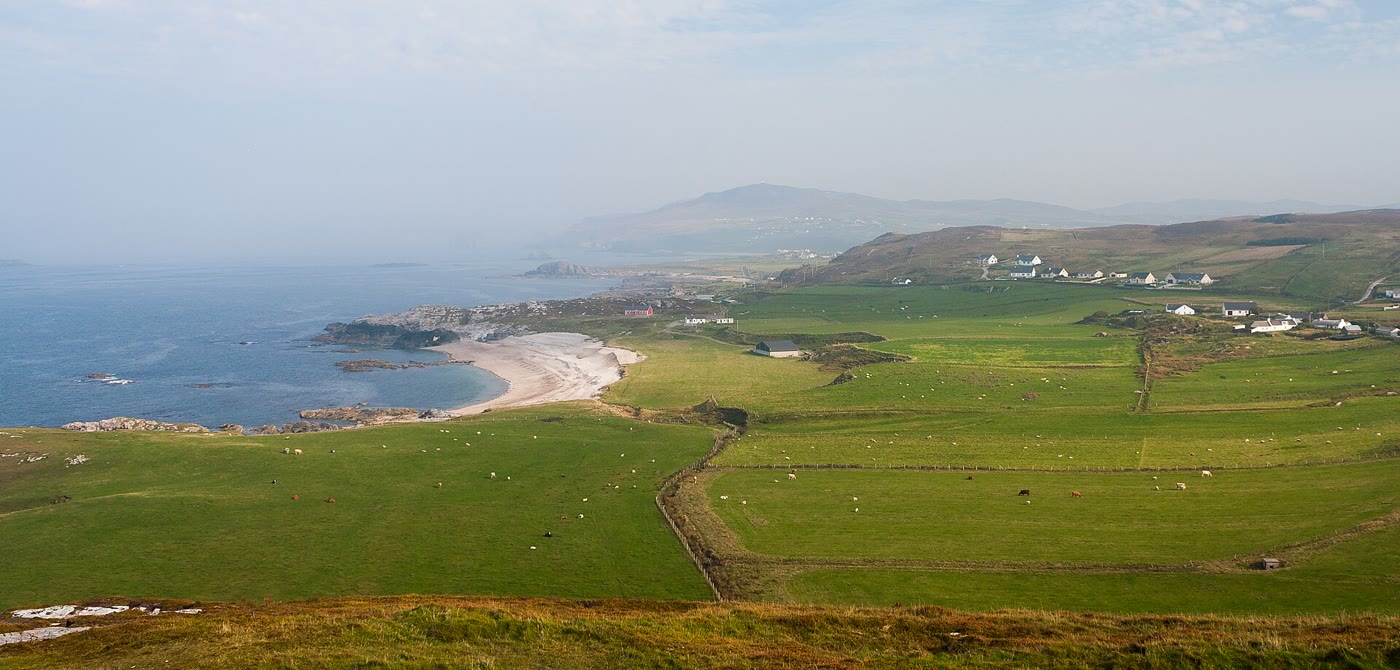
\includegraphics[width=\linewidth]{images/book5/b3-raised-beach-malin.jpg}

{\scriptsize 爱尔兰北部马林角的巴利希林抬升海滩：
旧岸线的圆砾滨脊随冰盖融化后陆地的抬升而高出海面。
照片：A.~F.~Borchert, CC BY-SA 4.0。}
\end{minipage}
\end{inthefield}
% ledger: photo:b3-raised-beach

\section{全地幔对流及其深部结构}

地幔究竟是作为一层对流，还是以
\qty{670}{km} 间断面为界分为上下两层对流？层析成像（\cref{ch:b3:seismology-imaging}）
可部分作答：有些板片在间断面之上平卧，另一些
穿过间断面没入下地幔，因而物质穿越间断面，两层之间
并非彼此密封。黏度随深度增大，使下地幔流动更为迟缓，
板片进入下地幔后减速并增厚。

地幔底部，层析成像显示出两个宽广的低 S 波速区，
分别位于非洲之下和太平洋之下，即大型低剪切波速省
（LLSVP）。它们很可能在化学成分上与其上方的地幔不同，
且密度更大，更像堆积体而非热地幔柱。过去数亿年间的大火成岩省与
金伯利岩大多喷发于其边缘上方，
仿佛地幔柱从堆积体边缘升起，那里正是地幔底部热边界
层被推抵堆积体的地方。
% ledger: st12:llsvp

\section{练习}

\begin{exercise}[$\star$]\label{exo:b3:mantle-convection:1}
求厚度为 \qty{670}{km} 的上地幔层的\omterm{def:b3:mantle-convection:rayleigh}{瑞利数}，其中
$\rho = \qty{3500}{kg.m^{-3}}$, $g = \qty{9.9}{m.s^{-2}}$, $\alpha =
\qty{3e-5}{K^{-1}}$, $\Delta T = \qty{1000}{K}$, $\kappa =
\qty{e-6}{m^2.s^{-1}}$ 及 $\eta = \qty{5e20}{Pa.s}$。对于自由滑移边界，
该值是临界值的多少倍？
\end{exercise}

\begin{exercise}[$\star$]\label{exo:b3:mantle-convection:2}
求黏度为 \qty{e21}{Pa.s}、剪切模量为
\qty{7.7e10}{Pa} 的地幔的\omterm{def:b3:mantle-convection:maxwell}{麦克斯韦时间}（以年计）。地幔对每日两次的地球潮汐、
冰盖融化以及
板片下沉的响应，分别是弹性还是黏性？
\end{exercise}

\begin{exercise}[$\star$]\label{exo:b3:mantle-convection:3}
已知 $\eta = \qty{e21}{Pa.s}$，$\rho = \qty{3300}{kg.m^{-3}}$ 及 $g =
\qty{9.8}{m.s^{-2}}$，求均匀半空间
在波长为 1000 和 \qty{3000}{km} 的载荷下的松弛时间。哪一种恢复更快？
\end{exercise}

\begin{exercise}[$\star$]\label{exo:b3:mantle-convection:4}
已知 $g = \qty{9.8}{m.s^{-2}}$，$\rho_m = \qty{3300}{kg.m^{-3}}$，$\rho_w =
\qty{1030}{kg.m^{-3}}$, $\alpha = \qty{3.1e-5}{K^{-1}}$, $T_m - T_0 =
\qty{1450}{K}$，$\kappa = \qty{0.8e-6}{m^2.s^{-1}}$ 及 \qty{1}{Ma} $=
\qty{3.156e13}{s}$。求 \qty{50}{Ma} 时的\omterm{prop:b3:mantle-convection:ridge-push}{洋脊推力}，它比
\qty{4.6e13}{N.m^{-1}} 的板片拉力小多少倍？
\end{exercise}

\begin{exercise}[$\star\star$]\label{exo:b3:mantle-convection:5}
一团直径为 \qty{10}{km}、温度比外界高 \qty{300}{K} 的地幔团，
以速度 $\rho g\alpha\Delta Td^2/\eta$ 上升（取 $\rho =
\qty{3300}{kg.m^{-3}}$, $g = \qty{9.8}{m.s^{-2}}$, $\alpha = \qty{3e-5}{K^{-1}}$,
$\eta = \qty{e21}{Pa.s}$，$\kappa = \qty{e-6}{m^2.s^{-1}}$）。(a) 求其
穿越自身尺度的上升时间，以及扩散时间 $d^2/\kappa$，并证明
二者之比即其\omterm{def:b3:mantle-convection:rayleigh}{瑞利数}。(b) 它先上升还是先冷却？(c)
它要多大，其\omterm{def:b3:mantle-convection:rayleigh}{瑞利数}才能达到 657.5？
\end{exercise}

\begin{exercise}[$\star\star$]\label{exo:b3:mantle-convection:6}
对于深度为 \qty{2891}{km}、$\mathrm{Ra} = \num{e7}$ 的一层，取 $\kappa =
\qty{e-6}{m^2.s^{-1}}$, $k = \qty{3.1}{W.m^{-1}.K^{-1}}$, $\Delta T =
\qty{1450}{K}$ 及 $\mathrm{Ra}_c = 657.5$，求边界层
厚度、\omterm{def:b3:mantle-convection:nusselt}{努塞尔数}、以 \unit{cm/\text{年}} 计的速度尺度以及
热流。
\end{exercise}

\begin{exercise}[$\star\star$]\label{exo:b3:mantle-convection:7}
某虚构热点隆起的截面积（垂直于热点轨迹）为 \qty{8e8}{m^2}，
其上板块以 \qty{9}{cm/\text{年}} 运动。已知 $\rho_m - \rho_w =
\qty{2270}{kg.m^{-3}}$，求其浮力通量，并取 $c_p =
\qty{1170}{J.kg^{-1}.K^{-1}}$ 与 $\alpha = \qty{3.1e-5}{K^{-1}}$，求其热流量。
它占地球 \qty{46.7}{TW} 的比例是多少？
\end{exercise}

\begin{exercise}[$\star\star$]\label{exo:b3:mantle-convection:8}
半径为 \qty{400}{km} 的地幔柱头，比地幔轻
\qty{30}{kg.m^{-3}}，在黏度为 \qty{e21}{Pa.s} 的地幔中上升。利用
斯托克斯定律，求其以 \unit{m/\text{年}} 计的速度，以及上升
\qty{2000}{km} 所需的时间。
\end{exercise}

\begin{exercise}[$\star\star$]\label{exo:b3:mantle-convection:9}
某地区在 \qty{10}{ka} 前冰盖融化时曾下沉 \qty{300}{m}，
并以 $\tau = \qty{4.4}{ka}$ 的时间常数松弛。求今日残余的下沉量以及
当前的隆升速率，并与在
于默奥附近测得的 \qty{10.3}{mm/\text{年}} 相比较。
\end{exercise}

\begin{exercise}[$\star\star\star$]\label{exo:b3:mantle-convection:10}
(a) 由 $F_{rp}$ 的表达式（取自
\cref{prop:b3:mantle-convection:ridge-push} 的证明），证明第一项
$\tfrac12(\rho_m - \rho_w)gw^2$，即为括号中的第二项。(b) 证明
$\int_0^\infty x\operatorname{erfc}x\,\mathrm dx = 1/4$，并用分部积分法。
(c) 取练习 4 的数值，求 \qty{100}{Ma} 时的两项。
\end{exercise}

\begin{exercise}[$\star\star\star$]\label{exo:b3:mantle-convection:11}
证明 $f(k) = (\pi^2 + k^2)^3/k^2$ 在 $k = \pi/\sqrt2$ 处取最小值，其中
此时其值为 $27\pi^4/4$。由此推出对流环流刚出现时一对对流环流的宽度，
以 $d$ 为单位，并求单个对流环流的宽度。
\end{exercise}

\begin{exercise}[$\star\star\star$]\label{exo:b3:mantle-convection:12}
一块长 \qty{6000}{km} 的板块，以 \qty{6}{cm/\text{年}} 的速度在
厚 \qty{150}{km}、黏度为 \qty{e20}{Pa.s} 的地幔层之上运动，其底部静止。(a)
求以 \unit{MPa} 计的\omterm{def:b3:mantle-convection:basal-drag}{底部拖曳力}，以及单位板块长度上的
阻力。(b) 与\omterm{prop:b3:mantle-convection:ridge-push}{洋脊推力} \qty{3.8e12}{N.m^{-1}} 及板片拉力
\qty{4.6e13}{N.m^{-1}} 相比较。(c) 若板片拉力的十分之一
传递至板块，则阻力与驱动力平衡时的速度为多少？
\end{exercise}

\section{问题：阿尔多湖的回弹}

\begin{problem}[{周末问题——虚构湖盆的回弹，
其下方地幔的黏度，以及该黏度所允许的
对流}]
\label{pb:b3:mantle-convection:1}
% values: calc/ch06.py; gia_relaxation.py, convection_scaling.py
阿尔多湖是一座虚构的湖泊，充满一个直径 \qty{250}{km} 的盆地，由
冰盖筑坝拦截，水深 \qty{300}{m}，持续约五万年。一万四千年前，
冰坝溃决，湖水在数周内排空。其
形成时水平的最高岸线如今已倾斜；湖盆中残留的几个小湖，
其已测定年代的岸线给出排水以来中心的隆升量，
相对于几乎未动的湖缘：

\smallskip
\begin{center}\small
\begin{tabular}{lcccccc}
\hline
排水以来的时间（ka） & 1 & 2 & 4 & 6 & 9 & 14\\
中心隆升量（米） & 11.5 & 21.6 & 38.0 & 50.5 & 64.0 & 77.2\\
\hline
\end{tabular}
\end{center}
\smallskip

取 $\rho_w = \qty{1000}{kg.m^{-3}}$、$\rho_m = \qty{3300}{kg.m^{-3}}$、$g =
\qty{9.8}{m.s^{-2}}$、\qty{1}{\text{年}} $= \qty{3.156e7}{s}$，并将地幔视为
均匀黏性半空间。

\medskip\noindent\textbf{第一部分——载荷。}
\begin{enumerate}
  \item 求湖水对湖底的压强。
  \item 在均衡平衡时，求湖底的下沉量，并说明
        为何式中出现的是地幔密度而非地壳密度。
  \item 将湖泊视为圆盘，求湖水的质量。
  \item 解释为何现今最高岸线发生倾斜，并求
        由湖缘至中心的平均坡度，以米每千米计。
  \item 将下沉视为一个谐波，其下沉的半波，自
        $-\lambda/4$ 至 $\lambda/4$ 之间，恰覆盖湖泊。求 $\lambda$ 及 $k =
        2\pi/\lambda$。
  \item 此载荷下方的流动，在多大深度上衰减了
        $e$ 倍？
\end{enumerate}

\medskip\noindent\textbf{第二部分——弛豫时间。}
\begin{enumerate}[resume]
  \item 假设湖泊已达到平衡，求表中每个时刻
        残留的下沉量。
  \item 证明：若下沉量按指数规律衰减，则其对数
        随时间线性下降。
  \item 由时刻 1 与 \qty{14}{ka} 求 $\tau$。
  \item 用该 $\tau$ 预测 \qty{6}{ka} 时的隆升量，并与
        表中数值比较。
  \item 求今日残留的下沉量，以及中心当前的隆升速率，
        以 \unit{mm/\text{年}} 计。
  \item 尚待发生的隆升量为多少？
  \item 再过多少年，隆升速率将降至
        \qty{0.5}{mm/\text{年}} 以下？
\end{enumerate}

\medskip\noindent\textbf{第三部分——黏度。}
\begin{enumerate}[resume]
  \item 由 $\tau$ 求半空间的黏度。
  \item 将其与芬诺斯堪的亚下方所测得的上\omterm{def:b3:mantle-convection:gia}{地幔黏度} \num{3.4e20}
        至 \qty{1e21}{Pa.s} 相比较。
        阿尔多湖的回弹取样于地幔的哪一部分？
  \item 取该黏度，求波长为
        \qty{3000}{km} 的载荷的弛豫时间。为何同等尺度的真实冰盖
        会比此更缓慢地弛豫？
  \item 若计入弹性岩石圈（本题忽略之），它对
        直径仅 \qty{250}{km} 的载荷的回弹有何影响？
  \item 取 $\mu = \qty{7.7e10}{Pa}$，求地幔的
        \omterm{def:b3:mantle-convection:maxwell}{麦克斯韦时间}，并说明采用黏性模型是否合理。
  \item 检验第 7 题的假设：湖泊存在期间，
        已达到的平衡下沉量占比为多少？
  \item $\log_{10}\eta$ 会变化多少，若取 $\lambda$ 为
        \qty{250}{km}？
\end{enumerate}

\medskip\noindent\textbf{第四部分——对流。} 取一厚 \qty{670}{km} 的上地幔层，
其 $\rho = \qty{3700}{kg.m^{-3}}$、$g =
\qty{9.9}{m.s^{-2}}$、$\alpha = \qty{3.1e-5}{K^{-1}}$、$\Delta T =
\qty{1450}{K}$、$\kappa = \qty{e-6}{m^2.s^{-1}}$、$k = \qty{3.1}{W.m^{-1}.K^{-1}}$
并取第三部分中的黏度。
\begin{enumerate}[resume]
  \item 求该层的\omterm{def:b3:mantle-convection:rayleigh}{瑞利数}。
  \item 它是临界值的多少倍（$\mathrm{Ra}_c = 657.5$）？
  \item 求边界层厚度与\omterm{def:b3:mantle-convection:nusselt}{努塞尔数}。
  \item 以 \unit{cm/\text{年}} 计算速度标度，并与板块
        速度 1 至 \qty{7.5}{cm/\text{年}} 相比较。
  \item 求热流，并给出它低于地球平均值
        \qty{92}{mW.m^{-2}} 的两个原因。
  \item 以 $\log_{10}$ 形式给出阿尔多湖下方上地幔的黏度
        $\eta$，单位为 \unit{Pa.s}。
\end{enumerate}
\end{problem}
